\chapter{Geologi}

For at kunne dimensionere et fundament, er det vigtigt at have en grundlæggende viden om det materiale, der arbejdes med, altså hvilken jord, samt dets egenskaber og geologien i området. I det følgende vil der derfor foretages en beskrivelse af Aalborgs geologi, samt en beskrivelse af jorden og dets styrkeparametre.

\section{Aalborgs geologi}

Bla bla...

\section{Jord}
\subsection{Beskrivelse af jord og jordtyper}
Jord er en massebetegnelse, da der findes mange forskellige typer af jordarter. Der findes to hovedgrupper af jord; rene mineraljordarter og organiske jordarter. 
\newline \indent{     }  De rene mineraljordarter kan være sorterede eller usorterede. Mineraljordarterne kan blive sorteret ved vand- og vindaflejring, og kan blive til det, der kendes som grus, sand, silt og ler. De usorterede mineraljordarter aflejres primært ved gletsjeraflejring, og betegnes som morænejordarter kaldet till.\citep{jordarter}
\newline \indent{     }  Organiske jordarter består af organisk materiale i form af plante- eller dyrerester. Disse jordarter kendes som muld, tørv, gytje mm.\citep{miljo}
\newline \indent{     }  De forskellige jordtyper har forskellige egenskaber. Egenskaberne afhænger af kornstørrelserne, som angives ved kornets diameter, og herved kan de inddeles i kornfraktioner\citep{geoteknik}. For eksempel ses inddelingen af kornstørrelserne for nogle mineraljordarter på Figur \ref{fig:kornstorrelser} .

\begin{figure}[htbp] \centering
	\begin{minipage}[b]{0.48\textwidth}\centering
		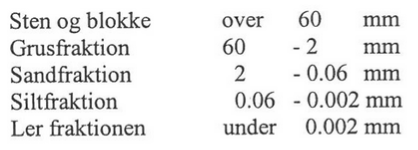
\includegraphics[width=1.0\textwidth]{billeder/kornetsdiameter.png}
		\caption{Inddeling af kornstørrelser for mineraljordarter (KILDE)}
		\label{fig:kornstorrelser}
	\end{minipage}\hfill
\end{figure}

\subsection{Jordtypernes udseende og dannelse}
Grus-  og sandjordarter skabes ved forvitring og erosion af materiale fra faste bjergarter. Materialet bliver herefter transporteret og aflejret via vind eller vand. Dette gør, at deres sammensætning bestemmes af udgangsmaterialet, men i lige så høj grad af transportmåden og transporttiden. Transporttiden kan gøre, at bløde dele af materialet opløses, samt at materialet får en afrundet kornform, og dette giver en mindre friktionsvinkel. Den relative store kornstørrelse ved grus og sandjordarter gør, at de har et groft porenet, hvilket medvirker, at vandet bevæger sig let i materialet,  dvs. at permeabiliteten er stor. Samtidig ved belastning af materialet sker der en vandudpresning, hvilket er en hurtig konsolidering.\citep{jordarter}
\newline \indent{     }  Grus- og sandjordarters styrkeegenskaber afhænger af friktionen mellem kornene, som afhænger af kornenes lejringstæthed, materialets enskornethed og kornenes enkelte form; om de er skarpkantet eller afrundet.\citep{jordarter} 
\newline \indent{     }  Lerjordarter har alle et bestemt indhold af lermineraler. Indholdet af disse har en betydende indflydelse på lerjordartens egenskaber, også selvom de ikke udgør størstedelen af jordarten. Lermineralerne bliver til ved en kemisk forvitring af faste bjergarter. De mest betydende grupper af lermineraler er; kaolinit, smectit, illit og chlorit. Den kemiske sammensætning af lermineralerne kan være meget forskellige og har en stor betydning for de fysiske egenskaber.\citep{jordarter} Alle lermineralerne kan optage vandmolekyler, hvilket gør, at lerjordarter kan indeholde meget vand. Betydningen af vandet kan fysisk ses ved tilsætning af vand til lerjordarterne, som gør at de sveller og ligeledes svinder ved tørring. Hvis lerpartiklerne er placeret med kort afstand til hinanden, vil dette give jordarten en større styrke.\citep{jordarter}  Ved at smadre jordarten formindskes jordartens styrke, men en del af denne styrke kan jordarten genvinde efter noget tid. \citep{jordarter}
\newline \indent{     }  Morænejordarter er typisk usorterede mineraljordarter, og kan derfor bestå af flere forskellige kornstørrelser. Fordelingen af dem kan skifte inden for korte afstande. Morænejordarter har normalt gode styrke- og deformationsegenskaber, da de er forbelastede.\citep{jordarter}
\newline \indent{     }  Organiske jordarters egenskaber er afhængige af de organiske bestanddeles art. De forskellige typer af organiske jordarter bliver dannet forskellige steder. Tørv og gytje bliver for eksempel dannet i moser, søer, bugter, fjorde mm, og dets styrke er ikke høj. Dette skyldes, at disse indeholder store mængder vand, da der ikke er faste partikler og at organiske materialer forsvinder med tiden. \citep{jordarter}

\subsection{Jords styrke og stivhed}
Jord betragtes, på lige fod med beton, stål osv, som et byggemateriale, da dens fysiske egenskaber er vigtige for konstruktions dimensionering.\citep{DGF} 
\newline \indent{     }  Jordarterne har meget forskellige styrker, og inden for geoteknik kan jordarterne inddeles i to forskellige typer. Den ene type er friktionsjord, for eksempel sand og grus. Den anden er kohæsionsjord med et indhold af mere end 10\% lerfraktion. 
Friktionsjord er under stabil lejring næsten usammentrykkeligt, og hvis deformationer finder sted forskydninger eller gnidninger kornene imellem.\citep{DGF}
\newline \indent{     }  I kohæsionsjord kan kornskelettet være stabilt ved åbne strukturer, men kun ved små deformationer og belastninger, afhængig af forbelastning. Ved store belastninger er disse jordarter sammentrykkelige.
\newline \indent{     }  Med hensyn til jordarters styrke, benyttes begreberne træk- og trykstyrke normalvis ikke. I stedet for anvendes forskydningsstyrken. Denne anvendes da der ved brud i jorden, sker en forskydning af jordmasser. Når der sker et sådant brud, virker der normal- og forskydningsspændinger langs brudlinjen.\citep{geoteknik} Forskydningsspændingen virker som en reaktion på jordmassens bevægelse nedad, og derfor er denne rettet skråt op ad. Normalspændingen, også kaldet brudspændingen, står vinkelret på brudlinjen, og regnes positiv ved tryk. Det vil være fordelagtigt at dele spændingen op i to bidrag; den effektive brudspænding og poreovertryk, som er trykket i porerne\citep{geoteknik}. Dette er illustreret på Figur \ref{fig:poretrykket}. 

\begin{figure}[htbp] \centering
	\begin{minipage}[b]{0.48\textwidth}\centering
		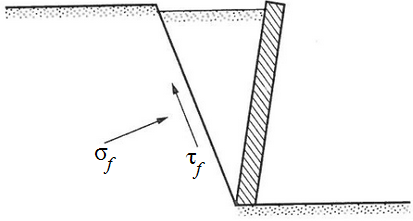
\includegraphics[width=1.0\textwidth]{billeder/poretrykket.png}
		\caption{BILLEDTEKST}
		\label{fig:poretrykket}
	\end{minipage}\hfill
\end{figure}

For at finde brud i jord bruges en skæreboks, som er illustreret på Figur \ref{fig:forskudningsspanding}. Jordprøven lukkes inde i en kasse, som lodret kan lastes med en varierende normalkraft. Kassen er delt vandret på midten, og ved at trække i øverste halvdel skabes et veldefineret vandret brud. Derved kan værdierne for brud- og forskydningsspænding måles.\citep{DGF}

\begin{figure}[htbp] \centering
	\begin{minipage}[b]{0.48\textwidth}\centering
		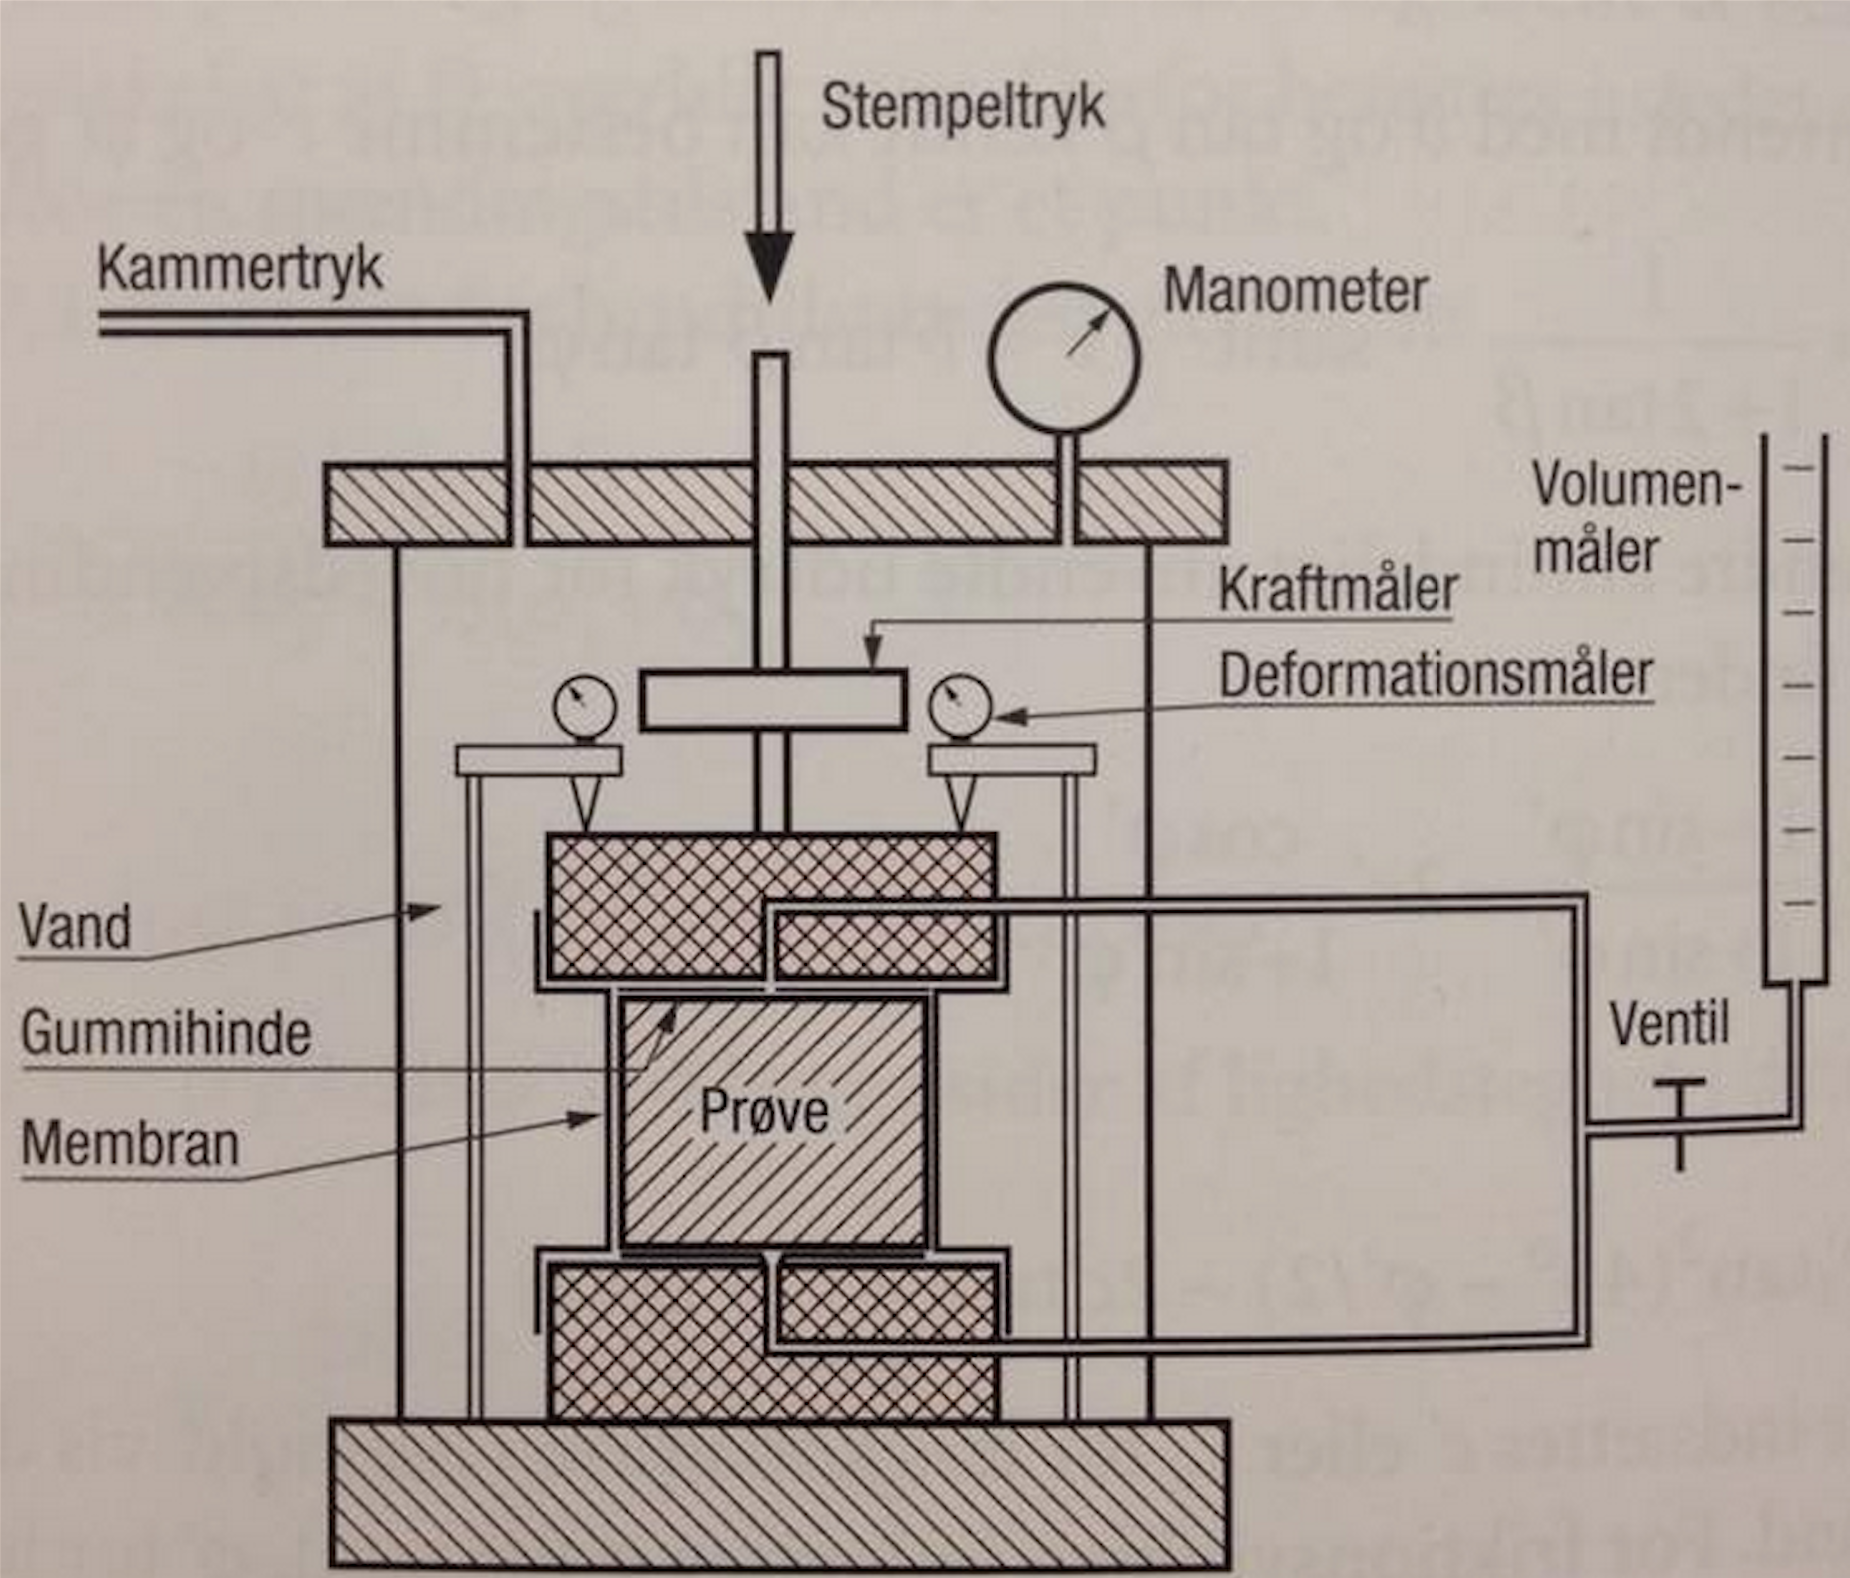
\includegraphics[width=0.8\textwidth]{billeder/forskud.png}
		\caption{BILLEDTEKST}
		\label{fig:forskudningsspanding}
	\end{minipage}\hfill
\end{figure}

\indent{     }  I kassen er jordprøven isoleret fra toppen og bunden via filtersten. Disse gør det muligt at kontrollere poretrykket, og således bestemme den effektive brudspænding. Ved forsøget findes der, at forskydningsspændingen består af to dele; kohæsionen og et friktionsbidrag. Kohæssionen er et konstant bidrag, og friktionsbidraget er proportionalt med den effektive brudspændning. Sammenhængen her kaldes for jordens brudbetingelse.\citep{geoteknik}
\newline \indent{     }  Friktionsvinklen er et mål for jord styrke. Friktionsvinklen er vidt forskellige alt efter jordtype, hvilket er illustreret på Figur \ref{fig:friktionsvinkler}.   

\begin{figure}[htbp] \centering
	\begin{minipage}[b]{0.48\textwidth}\centering
		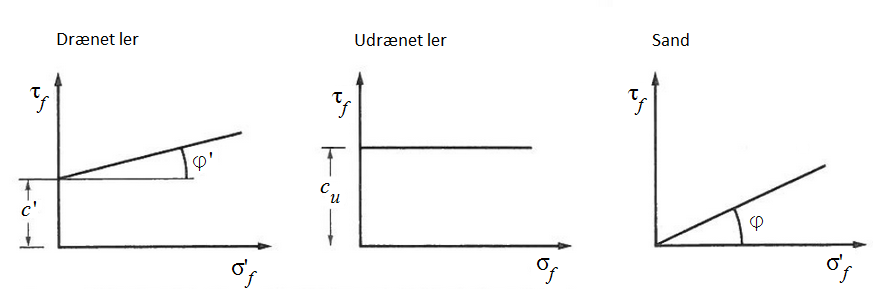
\includegraphics[width=1.0\textwidth]{billeder/friktionsvinkeller.png}
		\caption{Brudbetingelser for ler og sand \citep{geoteknik}}
		\label{fig:friktionsvinkler}
	\end{minipage}\hfill
\end{figure}
